\section{Experiments and what they establish}
\label{sec:experiments}

The experiments serve three different purposes: regression and source-proof
checking, controlled local timing, and falsification of overly broad
optimization claims. Their scopes should not be mixed. The principal
environment was Python 3.12.14 on Linux with Regina 7.4 for optional explicit
topological checks. Exact commands, versions, source hashes, raw timing
samples, and the saved proof objects are included in the package.

\subsection{Whole-cut coverage on the retained corpus}

The unchanged corpus is
\smallpath{fast/marked_parallelity_research/corpus.json}, with 106 supplied
source/vector cases. Its SHA-256 is recorded in both audit reports. The
baseline was copied from the pinned commit before any edit; the modified
run used the new top adapter with the same existing terminal policies.

\begin{table}[htbp]
\centering
\begin{tabular}{@{}lrr@{}}
\toprule
Whole-cut result & Baseline & With top adapter\\
\midrule
Complete censuses & 85 & 92\\
Independently replayed complete censuses & 85 & 92\\
Inconclusive & 21 & 14\\
Three-handle exclusion & 10 & 0\\
Raw cancellation stall & 8 & 10\\
Raw ball cancellation obstruction & 3 & 4\\
\bottomrule
\end{tabular}
\caption{The certified terminal primitive gains seven cases and preserves
 all 85 previous successes. The redistribution of failure reasons records
 progress beyond the old three-handle gate. It does not turn remaining
 refusals into negative topological verdicts.}
\label{tab:coverage}
\end{table}

All ten former three-handle cases receive a complete top reduction. Seven
then reach a complete whole-cut census, listed in \cref{tab:new}. The other
three remain inconclusive. Fresh Regina metric cuts and handlebody checks
were run for all ten and agree with the retained explicit reference data.
Each of the three remaining cases contains a nonhandlebody piece according
to that explicit check. In the JSON, a genus value of $-1$ is the oracle's
nonhandlebody sentinel, not a negative topological genus.

\begin{table}[htbp]
\centering\small
\begin{tabular}{@{}p{0.66\textwidth}l@{}}
\toprule
Newly certified case & Census $(\text{genus},\text{multiplicity})$\\
\midrule
\path{pilot/interior_1_2/0} & $(1,2)$\\
\path{pilot/interior_2_3/0} & $(1,2)$\\
\path{pilot/interior_3_5/0} & $(1,1)$\\
\path{pilot/finite_trefoil_interior/0} & $(2,1)$\\
\path{interior_1_2/mixed} & $(0,2)$\\
\path{interior_3_5/mixed} & $(0,2)$\\
\path{finite_figureEight_interior/mixed} & $(0,1),(2,2)$\\
\bottomrule
\end{tabular}
\caption{All seven new version-6 certificates are saved with their exact
source/vector inputs and independently replayed. These are censuses of
specified cuts, including cuts of nontrivial knot exteriors.}
\label{tab:new}
\end{table}

The three remaining former exclusions are
\path{pilot/finite_figureEight_interior/0},
\path{interior_2_3/mixed}, and
\path{finite_trefoil_interior/mixed}. Among the new total of 92 successes,
85 have explicit stored-oracle comparisons. The seven very large binary
scale cases are checked by independent compressed replay and their retained
scale expectations rather than literal expansion. The audit wall times
include different checking work and were not collected as a paired speed
comparison; they support no overall speedup claim.

\subsection{Regression, scale, and adversarial proof checks}

Fifty focused integration and regression tests passed: nine new top-handle
tests, seven existing whole-cut tests, and 34 existing core, annulus,
bundle-kernel, and initial-source-reduction tests. Five further source-tree
tests and twelve forest-exchange tests also passed. These are 67 distinct
named methods, not a claim to have rerun every historical test in the
repository.

The top tests include an actual five-tetrahedron solid torus with an
interior loop edge, obtained by a 1--4 and a 2--3 move. Its isomorphism
signature is \code{fLHPccdedehspga}. A forged trace that treats the loop's
two contacts as one is rejected. Another source has five interior vertices
and a genuinely dependent rooting order; moving a dependent cancellation
to the front is rejected. Rank-address changes, source mismatches, repeated
IDs, omitted proofs, and schema downgrades are tested. Verifier calls also
succeed with the corresponding producer functions disabled.

The reusable template was specialized on all 64 vectors obtained with
coefficients $0,1,2,3$ in a compatible sphere, boundary-disk, and M\"obius
band fixture. All traces independently replayed; two different specialized
move choices occur. Separate scale tests at $1$, $2^{64}$, and $2^{16384}$
produce top certificates of exactly 193 bytes with the stated JSON
serialization, while the largest coordinate needs 16,385 bits. This is
evidence for the trace-size statement, not for constant total certificate
size.

The abstract forest prototype was compared with exhaustive tree and row
checks on 12,350 labelled small graph instances and 1,200 seeded general-row
instances. Tests include forced contractions, loops, parallel edges, exact
deficiency optimization, malformed rank witnesses, and 16,385-bit labels or
counts. These instances test the graph theorem and implementation; most
were not produced by three-manifolds.

\subsection{A controlled benchmark on actual source triangulations}

Starting from the one-tetrahedron layered solid torus, perform $q$ interior
1--4 moves, always choosing the tetrahedron with the fewest boundary
corners and then the lowest index. Use the empty normal vector. The resulting
actual source has
\[
 t=3q+1,\qquad h_2=4q,\qquad h_3=q.
\]
Six sizes, $q=1,4,16,64,128,256$, were measured. Geometry was constructed and
independently authenticated outside the scheduler timers. Both the faithful
old diagnostic scan and the queue produced top traces that independently
replayed at each size.

Each scheduling comparison used nine randomized paired samples, calibrated
batches, and an additional nine queue/queue A/A pairs. Five samples measured
the common source-incidence reconstruction, and five randomized pairs
measured source reconstruction plus scheduling. The scan keeps its original
full sorted scan and candidate-list construction. Normalizing its final
output is excluded from its timer, while the queue includes survivor output
and counters; this choice favours the scan.

\begin{table}[H]
\centering\small
\begin{tabular}{@{}rrrrrr@{}}
\toprule
$q$ & $t$ & Scan (ms) & Queue (ms) & Local ratio & Combined ratio\\
\midrule
1 & 4 & 0.00118 & 0.00434 & 0.27$\times$ & 1.01$\times$\\
4 & 13 & 0.00936 & 0.01670 & 0.56$\times$ & 0.94$\times$\\
16 & 49 & 0.16567 & 0.08763 & 1.89$\times$ & 0.98$\times$\\
64 & 193 & 3.04399 & 0.35683 & 8.53$\times$ & 1.20$\times$\\
128 & 385 & 11.20248 & 0.73123 & 15.32$\times$ & 1.46$\times$\\
256 & 769 & 47.09763 & 1.63552 & 28.80$\times$ & 1.94$\times$\\
\bottomrule
\end{tabular}

\caption{Ratios are scan median divided by queue median. The combined
stage reconstructs source incidence for both methods. It excludes initial
parallelity construction, source-proof authentication, and terminal
recognition. Values below one are regressions.}
\label{tab:timing}
\end{table}

\begin{figure}[H]
\centering
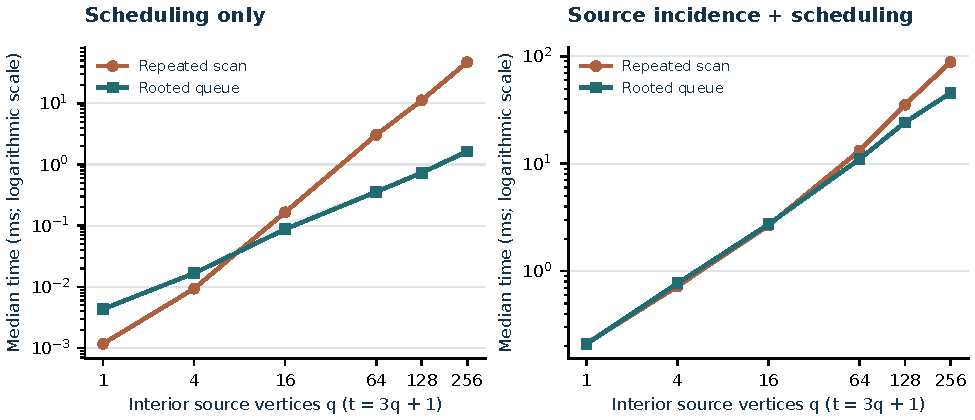
\includegraphics[width=\textwidth]{figures/local_scheduler.pdf}
\caption{Retained medians with interquartile bands. Common source work
substantially dilutes the scheduling gain. Both axes use logarithmic scales;
the two panels have different vertical ranges.}
\label{fig:timing}
\end{figure}

At $q=256$, the isolated medians are 47.098 ms for scanning and 1.636 ms
for the queue. Common source-incidence reconstruction alone takes 45.541 ms;
the directly measured combined medians are 88.425 ms and 45.655 ms. Thus
the observed ratios are $28.80$ and $1.94$, respectively. The queue has
greater constant overhead for the smallest inputs. A/A median paired ratios
range from 0.967 to 1.070; the $q=16$ ratio-of-medians A/A statistic is
noisier, 1.189. Small timing differences should not support a strong
interpretation. The largest effects are substantially larger than these
controls, but still concern a local Python implementation on a shared host.

There is also an exact asymptotic comparison independent of timing. With
$m=4q$, the old loop visits
\[
 qm-\frac{q(q-1)}2=\frac{7q^2+q}{2}
\]
rows. At $q=256$ this is 229,504 row visits and 457,462 actual interior-cap
membership tests. The queue performs 2,038 incidence updates; its explicit
upper bound including initialization is 9,426 endpoint inspections. The
old scan performs quadratic row-scan work on this genuine source family, while the new queue
has the linear structural bound of \cref{prop:cost}.

\subsection{The forest-planning experiment gives a negative result}

The native applicability audit fixes the maintained primal forest and
compares the abstract restricted planner with the ordinary rooted top queue
followed by raw core cancellation. On the 106 source cores, the restricted
planner completes 40 and refuses 66 because forced long rows already
contain a cap cycle. Ordinary core cancellation completes 100. The
restriction therefore misses 60 ordinary successes and adds no coverage.
On eight subdivided empty solid tori it completes only $q=1,2$, while
ordinary core cancellation completes all eight. This observed family is not
claimed as a theorem about every later subdivision.

These numbers concern the core before all attached bundles are resolved.
They are not the 92 whole-cut successes of \cref{tab:coverage}. In
particular, all ten former three-handle cores pass the ordinary core
consumer; the three remaining whole-cut refusals arise later.

All 114 source cores in the chain audit satisfy the uncapped
$A^{\mathsf T}B=0$ identity; 18 checks involve actual three-handles. The
mandatory set $\overline D$ is a cap forest in 40 corpus cases and two
subdivision cases. Every one has $\beta_2=0$, and the contracted rank
formula and source trace replay agree. The data do not empirically test
nontrivial forest variation: in every eligible case $|\overline D|=q$,
so the eight proposed edge orders yield the same tree. All full cores in
this audit have $\beta_2=0$. The invariance and positive-nullity statements
are supported by the proof and the explicit geometric family in
\cref{ex:geometric-cycle}, not by an overstated experimental claim.

\subsection{The exceptional-row quotient retains the missing information}

The fixed-forest quotient was checked on 21,304 ternary matrices with at
most three rows and columns, 4,096 binary $4\times3$ matrices, 3,375 legal
exceptional partitions of binary $3\times3$ matrices, and 2,000 seeded
larger matrices. Tests verify decision equivalence, exact canonical
stopping rows, lifted source schedules, ground handling, duplicate types,
and large coefficients. Separate replay verifies all 120 retained abstract
and native certificates without importing the producer.

For the ordinary fixed dual forest in the native corpus, all 106 short-row
graphs are forests. The quotient recovers the 100 complete cores and six
canonical stopping cores. In aggregate, 773 source rows reduce to 164
exceptional rows, and 809 occurring source columns reduce to 189 distinct
nonzero quotient types. The maximum exceptional-row count is nine, with
median one. All eight subdivision cores also complete. These are exact
structural compression measurements. Ordinary peeling already decides
these explicit matrices, so we claim no new measured runtime or coverage
gain from the quotient itself.
